\textbf{COLUNI 2023 -- Questão 31}\par\medskip Leia o texto a seguir.

\par

\textbf{Mortes por chuvas em 2022 já superam ano passado inteiro}

\par

Nos primeiros 5 meses de 2022, 457 pessoas morreram em desastres causados pelo excesso de chuva no Brasil, segundo levantamento da Confederação Nacional de Municípios (CNM) com base nos dados das defesas civis municipais. [...] O total de 457 óbitos representa um aumento de 57\% em relação a 2021, quando o número de mortos pela chuva no ano todo foi de 290 pessoas. Em 2019 o número de mortes pela chuva cresceu muito em relação aos anos anteriores. Foram 297 mortos em 2019 e 216 em 2020. Como comparação, entre 2014 e 2018 morreram menos de 100 pessoas por ano por causa da chuva (veja gráfico abaixo).

% COLUNI-AUTO-FIGURES-BEGIN
\begin{figure}[htbp]
\centering
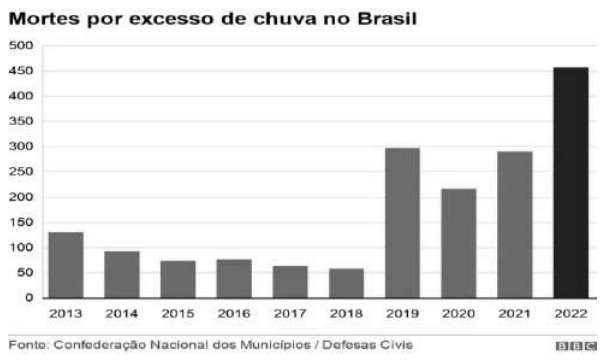
\includegraphics[width=0.95\linewidth]{static/simulados/coluni/figuras/2023/questao-31/figura-1.png}
\end{figure}
% COLUNI-AUTO-FIGURES-END

\par

Em um relatório sobre os danos causados pelo excesso de chuvas, a CNM aponta que, apesar dos desastres terem sido desencadeados pelo alto volume de precipitação, muitos dos problemas - incluindo mortes evitáveis - são resultado da falta de políticas públicas. [...] O maior desastre em número de óbitos de 2022 aconteceu em fevereiro em Petrópolis, no Rio de Janeiro, quando 233 pessoas morreram devido a deslizamentos e alagamentos causados pela chuva. [...] O Rio de Janeiro teve outro desastre em abril, quando as chuvas causaram deslizamentos que deixaram 20 mortos (11 mortos em Angra dos Reis, 7 em Paraty e 1 em Mesquita). Os estados do nordeste também foram fortemente afetados. Somente em Recife (PE), pelo menos 91 pessoas morreram na última semana de maio. Outras 26 pessoas morreram na Bahia no início do ano. A região nordeste também teve 1,2 milhão de pessoas afetadas pelas chuvas e pelo menos R\$ 3 milhões em prejuízo nos últimos 6 meses, com danos à pecuária, à agricultura, à indústria, ao comércio, aos sistemas de geração de energia, de abastecimento de água, de esgoto, de limpeza, de segurança pública, de controle de pragas, de transportes e de telecomunicações. Disponível     em:       https://epocanegocios.globo.com/Brasil/noticia/2022/06/mortes-por-chuvas-em-2022-ja-superam-ano-passado- inteiro.html. Acesso: em 01 Jun. 2022. (Adaptado)

\par

Considerando o elevado número de mortes ocorridas no Brasil em 2022 em função do excesso de chuvas, é CORRETO afirmar:

\begin{enumerate}
\item Trata-se de uma catástrofe natural e ocorre devido à localização subtropical que o país possui, estando
        associada à dinâmica atmosférica do Brasil que é diferente da dinâmica atmosférica global, pois refere-se a
        uma escala reduzida.
\item Poderiam ter sido completamente evitadas se todos os afetados pelas catástrofes tivessem respeitado as leis e
        as políticas públicas de contenção de tragédias naturais, pois no período de inverno essas tragédias sempre
        ocorrem.
\item Os locais onde ocorreram as tragédias são fortemente influenciados pelo regime hídrico dos rios que,
        estimulados pelo relevo de planície, possibilitam as inundações como ocorreram em Minas, Petrópolis, Bahia e
        Recife.
\item O elevado número de mortes ocasionadas pelo excesso de chuva está relacionado diretamente com o local de
        moradia e de ocupação das pessoas em áreas de encostas, onde a falta de infraestrutura urbana compromete
        a qualidade de vida dos moradores.\end{enumerate}
